\newpage
\subsection{Astrobiology}
\label{sec:Astrobiology-Results}

	\begin{figure}[H]
	\begin{center}
	\begin{minipage}[c]{.75\textwidth}
	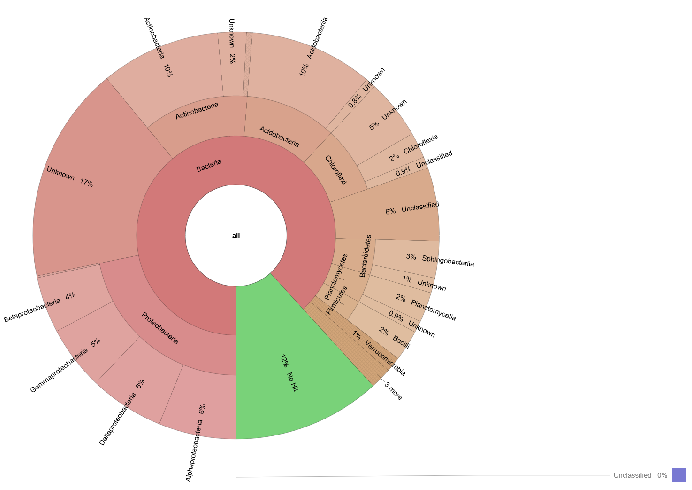
\includegraphics[width=1.2\textwidth]{./Figures/ConKrona.pdf}
	\caption{Sequencing results for the astrobiology control sample.}
	\label{fig:astro_hits1}
	\end{minipage}
	\hfill
	\begin{minipage}[c]{.75\textwidth}
	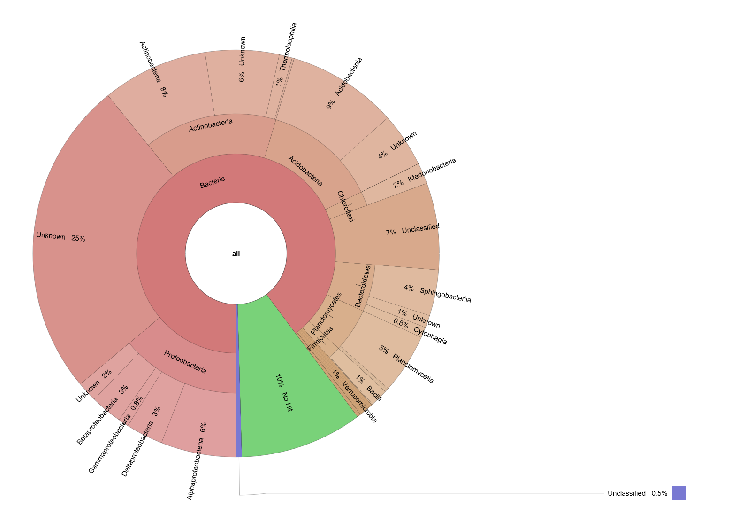
\includegraphics[width=1.2\textwidth]{./Figures/ExpKrona.pdf}
	\caption{Sequencing results for the astrobiology experimental sample.}
	\label{fig:astro_hits2}
	\end{minipage}
	\end{center}
	\end{figure} 
	
		\begin{figure}[H]
	\begin{center}
	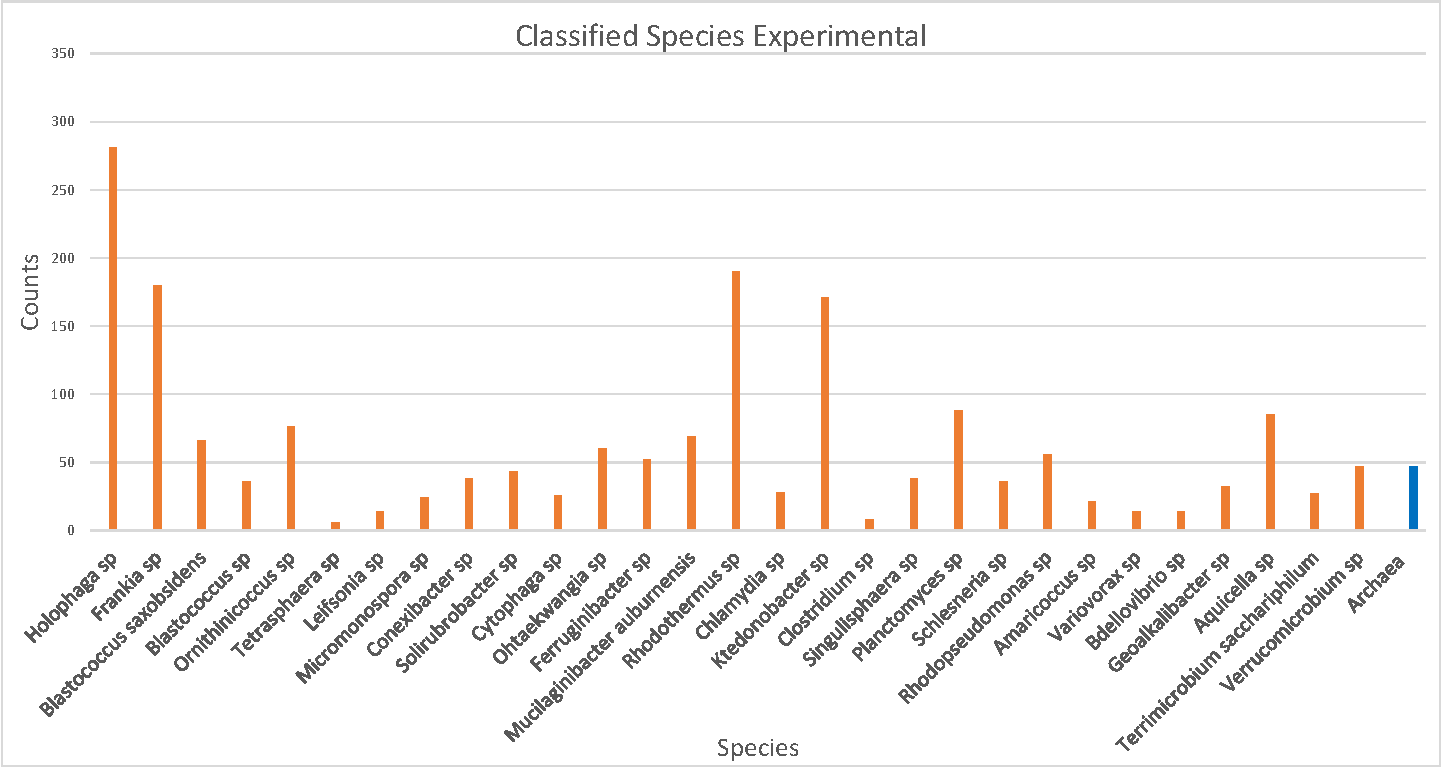
\includegraphics[width=1\textwidth]{./Figures/ClassifiedExp.pdf}
	\caption{Classified species captured in the experimental sample and not Identified in the control sample, orange are Bacteria and blue is the single Archaea species found.}
	\label{fig:astro_hits3}
	\end{center}
	\end{figure} 

	\begin{figure}[H]
	\begin{center}
	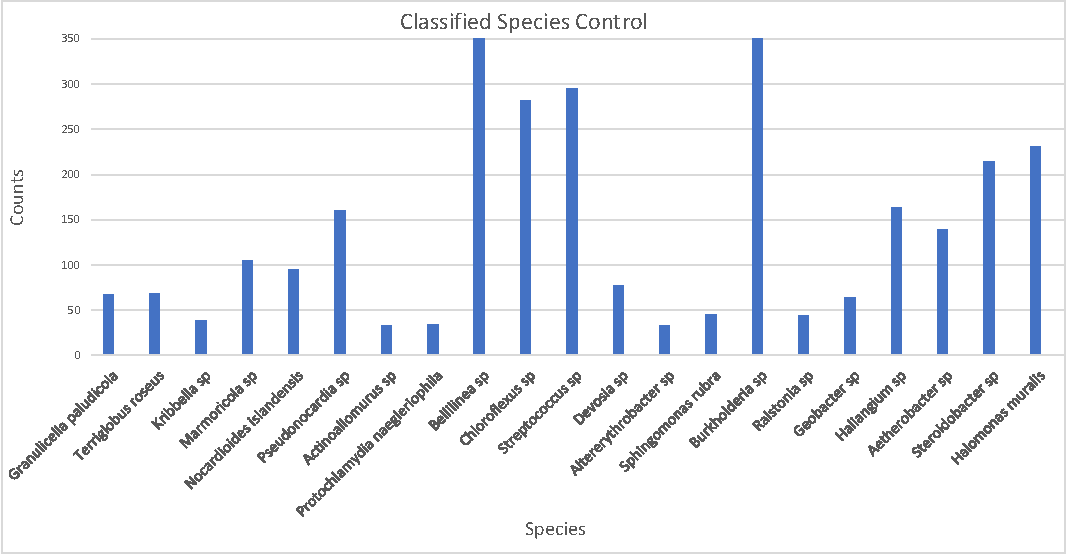
\includegraphics[width=1\textwidth]{./Figures/ClassifiedCon.pdf}
	\caption{Classified species identified in the control sample and not Identified in the experimental sample, all species found in the control sample are Bacteria.}
	\label{fig:astro_hits4}
	\end{center}
	\end{figure} 

	
As displayed in Figure~\ref{fig:astro_hits1} and Figure~\ref{fig:astro_hits2}, the RNA sequencing provided by RTL Genomics gives results that show a difference between the control and experimental samples.  Of interest is the presence of Archaea and various Bacteria in the experimental sample that are absent from the control sample.
Figure~\ref{fig:astro_hits3} shows the counts of all classified species captured in the experimental container not identified in the control container and Figure~\ref{fig:astro_hits4} shows the counts of all classified species identified in the control container and not identified in the experimental container.



